\section{Poiseuille flow with ring-molecules}
For the final task the goal was to perform Poiseuille flow simulation, where two stationary walls were placed on opposite sides of the domain. In addition a constant body force $F_{body} = 0.3$ was applied to all non-wall particles. The system contained $10$ ring molecules, each with 9 particles of type A, alongside fluid particles. The bond parameters were given as $K_S = 100$ and $r_S = 0.3$.

\subsection{Temperature and Energy Analysis}
The temperature history plot in Figure \ref{fig:poiseuille} hows a rapid initial equilibration followed by a steady increase, reaching approximately 40 units by the end of the simulation. This temperature rise is to be expected in a Poiseuille flow setup where kinetic energy is continuously added to the system by the body force.

\subsection{Flow Profile Analysis}
The velocity profile shows the characteristic parabolic shape expected for Poiseuille flow, with maximum velocity in the center of the channel and zero velocity at the walls. On top over the duration of the simulation this velocity stays constant. This confirms the correct implementation of the body force and wall boundary conditions.

\subsection{Molecule Distribution and Evolution}
The ring molecules show a distribution pattern across the channel:
\begin{enumerate}
	\item Initially randomly distributed, the rings form and then afterwards gradually migrate toward the center of the channel over time.
	\item The molecule distribution histogram shows higher concentrations near the center and decreased presence near the walls.
	\item The rings appear to maintain their circular structure throughout the simulation, showing the effectiveness of the bond implementation.
\end{enumerate}
The migration of ring molecules toward the center is a known effect as "cross-stream migration" or "tubular pinch effect." The primary reason for this migration is the balance between:
\begin{enumerate}
	\item Wall-induced migration: The interaction with walls creates an effective repulsive force pushing particles away from the walls.
	\item Shear-induced migration: The non-uniform shear rate across the channel, where it is the highest near walls and  lowest at center in Poiseuille flow, creates a driving force that moves particles from high-shear to low-shear regions.
\end{enumerate}
This effect is especially visible for structures like our ring molecules, as they experience different shear forces across their structure. The resulting hydrodynamic lift pushes them toward the center of the channel where the shear rate is minimal.

\begin{figure}[H]
	\begin{center}
		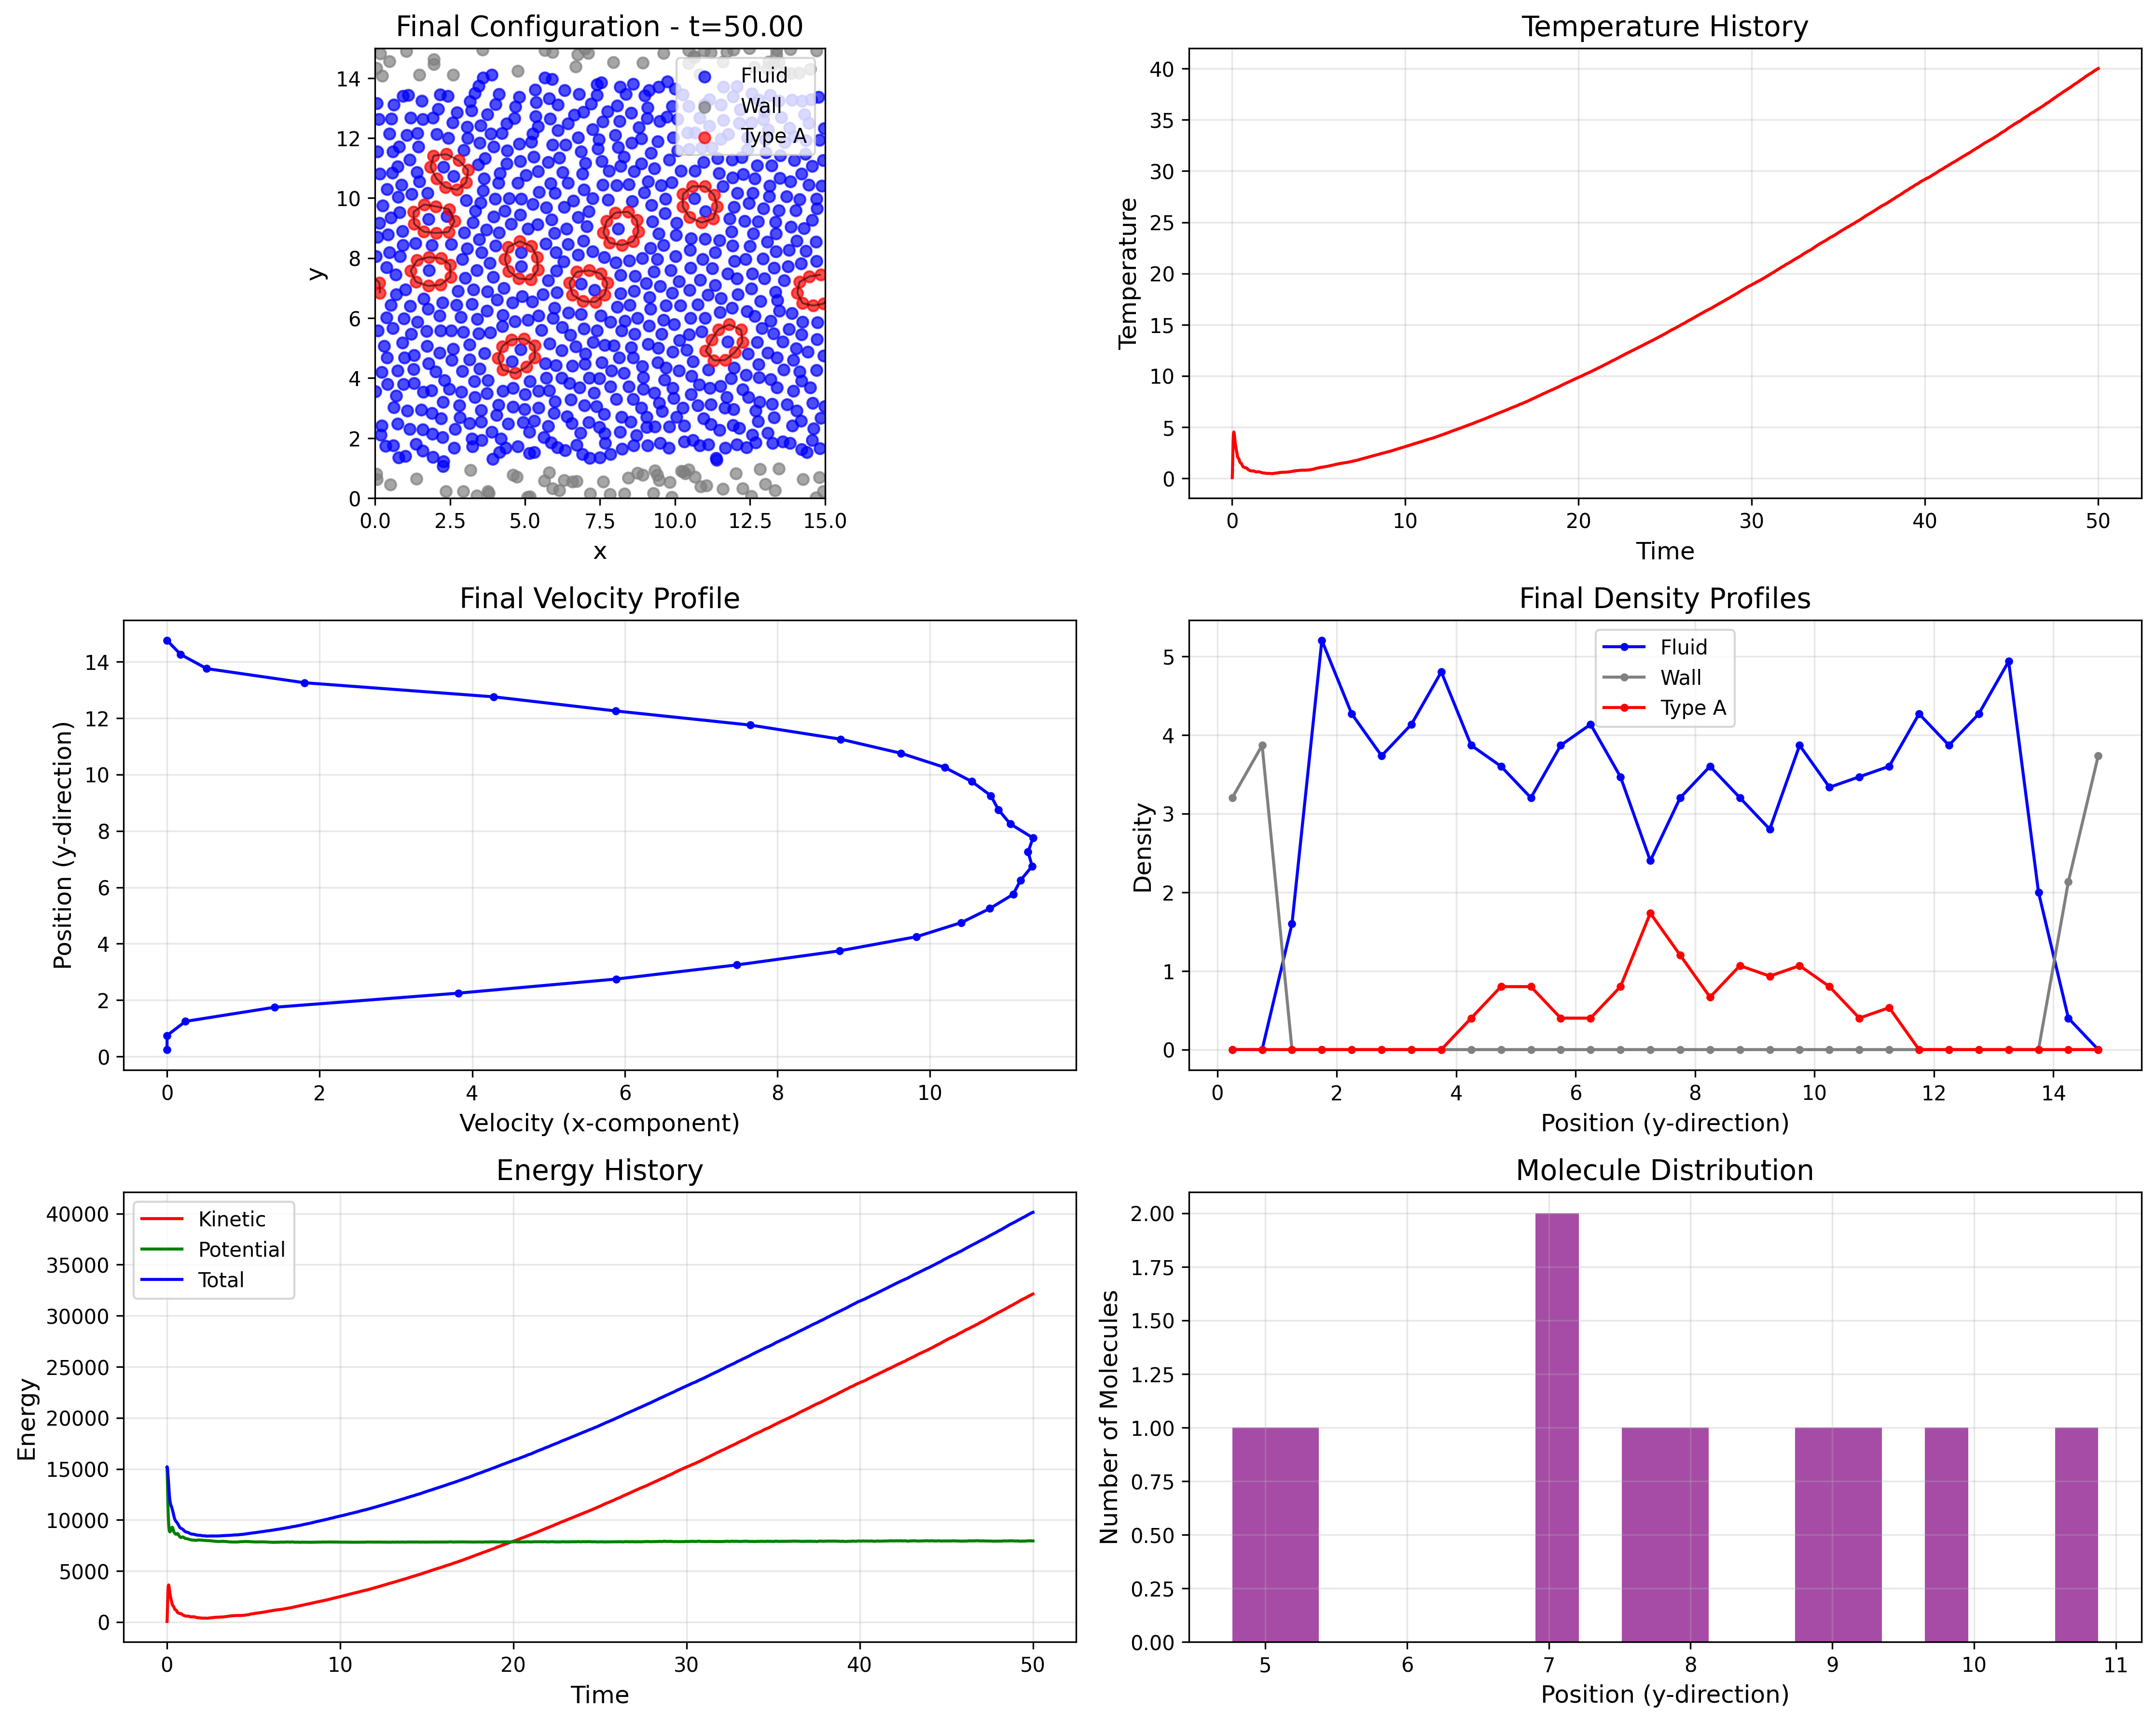
\includegraphics[width=0.95\textwidth]{figures/poiseuille_vis_final_0.01.png}
	\end{center}
	\caption{Poiseuille flow with $dt=0.01$ with $5000$ steps}\label{fig:poiseuille}
\end{figure}

\section*{Conclusion}
The DPD simulations that were performe successfully captured the expected behaviors of the Test, Couette and Poiseuille behaviors and flows for the latter two. The implementation of different types of moluces (chain and ring) showed the capability of DPD to model complex fluids with structured components.
Key findings include:
\begin{enumerate}
	\item The DPD thermostat effectively maintained system temperature around the desired value.
	\item Chain molecules in Couette flow aligned with the flow direction and showed a level of aggregation.
	\item Ring molecules in Poiseuille flow exhibited cross-stream migration toward the center of the channel. 
\end{enumerate}
These simulations showed the validity and potential of DPD as a simulation method that can capture complex phenomena  when molecular and continuum scales meet. The soft repulsive potentials and momentum-conserving thermostat make it particularly suitable for simulating soft matter and complex fluids.
